%!TEX root = ./main.tex

\section*{Appendix}

\section{Applications in Section~\ref{sec:covering}}
To apply Theorem \ref{thm:covering-formal} on specific problems, we need to determine the local-smoothness parameters for the multilinear extension.
\cite{Thang20:Online-Primal-Dual} provided these parameters for some broad classes of functions, in particular for polynomials with non-negative coefficients. Let $g_{\ell}: \mathbb{R} \rightarrow \mathbb{R}$ for $1 \leq \ell \leq L$
be degree-$k$ polynomials with non-negative coefficients and let $f:~\{0,1\}^{n}~\rightarrow~\mathbb{R}^{+}$ be the cost function
defined as $f(\vect{1}_{S}) = \sum_{\ell} b_{\ell} g_{\ell}\bigl( \sum_{e \in S} a_{e} \bigr)$ where $a_{e} \geq 0$ for every
$e$ and $b_{\ell} \geq 0$ for every $1 \leq \ell \leq L$.
Then the multilinear extension $F$ of $f$ is $(O(k \ln(d/\eta))^{k-1}, \frac{k-1}{k \ln(1 + 2d^{2}/\eta)})$-locally smooth.
We will use these parameters to derive the guarantees for the following problems.



%%% **************************
%%% **************************
%%% **************************

\subsection{Load Balancing}

\paragraph{Problem.}
Load balancing is a classic problem in discrete optimization with wide-ranging applications (for example, resource management in data centres).
This problem revolves around assigning jobs that arrive online to $m$ available unrelated machines while minimizing their maximum load.
Each arriving job $j$ reveals its machine dependent execution time $p_{ij}$ where $i \in \{1, m\}$ is the machine's index. The load $\ell_{i}$ of machine $i$ is the total processing time of the jobs assigned
to it. This load balancing problem is a well understood standard online problem and it has a tight competitive ratio of $\Theta(\log m)$ (\cite{BorodinEl-Yaniv05:Online-computation,Caragiannis08:Better-bounds}).

In our online setting with predictions, the jobs not only arrive with their machine dependent execution time $p_{ij}$, but their machine dependent prediction as well. Formally, $x_{ij} \in \{0,1\}$ indicates whether job $j$ is assigned to machine $i$, and the oracle provides $pred(x_{ij}) \in \{0,1\}$. We can formulate the online load balancing problem as a non-linear program. The objective is $\min \max_{i=1}^{m} \ell_{i} = \min \max_{i=1}^{m} \bigl(\sum_{j} p_{ij} x_{ij}\bigr)$, and the constraint is $\sum_{i=1}^{m} x_{ij} = 1$ which guarantees that each job $j$ is assigned to some machine $i$. Applying our framework for non-linear programs with covering constraints, Proposition~\ref{prop:load} follows.

\setcounter{theorem}{4}
\begin{proposition}
Algorithm~\ref{algo:covering} gives a
$O(\frac{1}{1 - \eta})$-consistent and $O\bigl((\log m) \log^{2} \frac{m}{\eta}\bigr)$-robust fractional solution
for the load balancing problem.
\end{proposition}
%
\begin{proof}
It is known that $\infty$-norm of a $m$-dim vector can be approximated by the $(\log m)$-norm,
in particular for $m \geq 2$,
$$
\|(\ell_{1}, \ell_{2}, \ldots, \ell_{m})\|_{\infty} \leq \|(\ell_{1}, \ell_{2}, \ldots, \ell_{m})\|_{\log m}
\leq m^{1/m} \|(\ell_{1}, \ell_{2}, \ldots, \ell_{m})\|_{\infty}
\leq 2 \|(\ell_{1}, \ell_{2}, \ldots, \ell_{m})\|_{\infty}.
$$
Hence, one can instead consider the objective of minimizing the  $(\log m)$-norm of the load vectors
while losing a constant factor of 2. More precisely, we consider the $(\log m)$-th power of the $(\log m)$-norm as the objective.
$$
\min \sum_{i=1}^{m} \biggl(\sum_{j} p_{ij} x_{ij}\biggr)^{\log m}
\qquad \text{s.t.} \qquad
\sum_{i=1}^{m} x_{ij} = 1 ~ \forall j
$$
%
The objective function is a polynomial of degree $\log m$. So its multilinear extension is \linebreak
$(O(k \ln(d/\eta))^{k-1}, \frac{k-1}{k \ln(1 + 2d^{2}/\eta)})$-locally smooth
with $k = \log m$ and $d = m$ (the maximal number of positive coefficients in a constraint).
Therefore, applying Theorem~\ref{thm:covering-formal}, the robustness (w.r.t the objective as  the $(\log m)$-th power of the $(\log m)$-norm)
is $O\bigl((\log m \log \frac{m}{\eta})^{\log m}\bigr)$.
Getting back to the $(\log m)$-norm objective by taking the $(\log m)$-root,
the robustness is  $O\bigl((\log m) \log^{2} \frac{m}{\eta}\bigr)$.
Hence, Algorithm~\ref{algo:covering} is $O(\frac{1}{1 - \eta})$-consistent and $O\bigl((\log m) \log^{2} \frac{m}{\eta}\bigr)$-robust.
\end{proof}

%%% **************************
%%% **************************
%%% **************************

\subsection{Energy Minimization in Scheduling}

\paragraph{Problem.}
Reducing carbon emissions is a global effort in which energy-efficient algorithms play an essential role. For example, \cite{Albers10:Energy-efficient-algorithms} and \cite{GuCaiZengZhangJinDai:2019} studied energy-efficient algorithms for scheduling.

Given $m$ unrelated machines, we need to assign jobs that arrive online. Each job $j$ has a release date $r_{j}$, a deadline $d_{j}$, and a vector of machine dependent processing times $p_{ij}$. Contrary to performance-oriented scheduling, our goal is to design an assignment policy which can minimize the total energy consumption of the execution. To achieve this, we can adjust the machines' speed $s_{ij}(t)$ during the time interval $[t,t+1)$ for the execution of job $j$. Every machine $i$ has a non-decreasing energy power function $P_{i}(\cdot)$. Typically, $P_{i}(z) = z^{k_{i}}$ for some constant $k_{i} \geq 1$. The execution's total energy is $\sum_{i} \sum_{t} P(\sum_{j} s_{ij}(t))$.

In the classic online setting, this problem is well understood: there exists an $O(k^{k})$-competitive algorithm (\cite{Thang20:Online-Primal-Dual}) where $k = \max_{i} \{k_{i}\}$
and this bound is tight up to a constant factor (\cite{Caragiannis08:Better-bounds}). In our extended study with predictions we represent this problem with the following non-linear program. The objective is $\min \sum_{i} \sum_{t} P(\sum_{j} s_{ij}(t))$ and the constraints are:
$$
\sum_{i=1}^{m} x_{ij} = 1,  \qquad \qquad \sum_{t = r_{j}}^{d_{j}-1} s_{ij}(t) \geq p_{ij} x_{ij}, \qquad  \qquad s_{ij}(t) \geq 0  \qquad \forall\ i,\ t
$$
where $x_{ij} \in \{0,1\}$ indicates whether job $j$ is assigned to machine $i$
and $s_{ij}(t) \geq 0$ denotes the speed of machine $i$ executing job $j$ during the time interval $[t, t+1)$.
The first constraint guarantees that job $j$ is assigned to some machine, and the second one ensures
that the job $j$ is completed on time (on the machine where the job is assigned). At the arrival of
job $j$, the prediction provides a solution $pred(x_{ij})$ and a speed $pred(s_{ij}(t))$ for $r_{j} \leq t \leq d_{j} - 1$.
Using our framework, we can deduce the following result.

\begin{proposition}
Algorithm~\ref{algo:covering} gives a
$O(\frac{1}{1 - \eta})$-consistent and $O\bigl(k^{k} \log^{k} \frac{m}{\eta}\bigr)$-robust fractional solution
for the energy minimization problem.
\end{proposition}
%
\begin{proof}
The objective function $\sum_{i} \sum_{t} P(\sum_{j} s_{ij}(t))$ is a polynomial of degree $k = \max_{i} k_{i}$;
so its multilinear extension is
$(O(k \ln(m/\eta))^{k-1}, \frac{k-1}{k \ln(1 + 2m^{2}/\eta)})$-locally smooth
(the maximal number of positive coefficients in a constraint $d = m$).
Therefore, applying Theorem~\ref{thm:covering-formal},
Algorithm~\ref{algo:covering} provides a $O(\frac{1}{1 - \eta})$-consistent and $O\bigl(k^{k} \ln^{k} \frac{m}{\eta}\bigr)$-robust
fractional solution.
\end{proof}



%%% **************************
%%% **************************
%%% **************************

\subsection{Online Submodular Mimimization}	\label{apix:sub-min}

\paragraph{Problem.} Submodular minimization is a widespread subject in optimization and machine learning (\cite{IwataFleischer01:A-combinatorial-strongly,Bachothers13:Learning-with,Bach16:Submodular-functions:,BalkanskiSinger:2020}). Let us consider the problem of minimizing an online monotone submodular function subject to covering constraints.
A set-function $f: 2^{\mathcal{E}} \rightarrow \mathbb{R}+$ is \emph{submodular} if
$f(S \cup e) - f(S) \geq f(T \cup e) - f(T)$ for all $S \subset T \subseteq \mathcal{E}$.
Let $F$ be the multilinear extension of a monotone submodular function $f$. Function $F$
admits two useful properties. First, if $f$ is monotone, then so is $F$. Second, $F$ is concave in
the positive direction, meaning that $\nabla F(\vect{x}) \geq \nabla F(\vect{y})$ for all $\vect{x} \leq \vect{y}$, where $\vect{x} \leq \vect{y}$ is defined as $x_{e} \leq y_{e} ~\forall e$.

To apply Algorithm~\ref{algo:covering}, we need to determine the local-smoothness parameters.
An important concept in studying submodular functions is the \emph{curvature}. Given a submodular
function $f$, the \emph{total curvature} $\kappa_{f}$ (\cite{ConfortiCornuejols84:Submodular-set-functions}) of $f$ is defined as
$
\kappa_{f} = 1 - \min_{e} \frac{f(\vect{1}_{\mathcal{E}}) - f(\vect{1}_{\mathcal{E} \setminus \{e\}})}{f(\vect{1}_{\{e\}})}.
$
Intuitively, the total curvature measures how far away $f$ is from being \emph{modular}. This concept of
curvature is used to determine both upper and lower bounds on the approximation ratios
for many submodular and learning problems (see \cite{ConfortiCornuejols84:Submodular-set-functions,GoemansHarvey09:Approximating-submodular,BalcanHarvey12:Learning-Submodular,Vondrak10:Submodularity-and-Curvature:,IyerJegelka13:Curvature-and-optimal,SviridenkoVondrak17:Optimal-approximation}).
The following lemma shows a useful property of the total curvature.

\setcounter{theorem}{7}
\begin{lemma}		\label{lem:curvature}
For any set $S$, it always holds that
$$
f(\vect{1}_{S}) \geq (1-\kappa_{f}) \sum_{e \in S} f(\vect{1}_{\{e\}}).
$$
\end{lemma}
\begin{proof}
Let $S = \{e_{1}, \ldots, e_{m}\}$ be an
arbitrary subset of $\mathcal{E}$. Let $S_{i} = \{e_{1}, \ldots, e_{i}\}$ for $1 \leq i \leq m$ and $S_{0} = \emptyset$.
We have
\begin{align*}
f(\vect{1}_{S})
&\geq  f(\vect{1}_{\mathcal{E}}) -  f(\vect{1}_{\mathcal{E} \setminus S})
= \sum_{i=0}^{m-1}  f(\vect{1}_{\mathcal{E} \setminus S_{i}}) - f(\vect{1}_{\mathcal{E} \setminus S_{i+1}})
\geq \sum_{i=1}^{m}  f(\vect{1}_{\mathcal{E}}) - f(\vect{1}_{\mathcal{E} \setminus \{e_{i}\}}) \\
&\geq (1 - \kappa_{f}) \sum_{i=1}^{m} f(\vect{1}_{e_{i}})
\end{align*}
where the first two inequalities are due to the submodularity of $f$, and the last inequality follows the definition of curvature.
\end{proof}

\setcounter{theorem}{6}
\begin{proposition}
Algorithm~\ref{algo:covering} gives a
$O(\frac{1}{1 - \eta})$-consistent and $O\bigl( \frac{\log (d/\eta)}{1 - \kappa_{f}} \bigr)$-robust fractional  solution
for the submodular minimization under covering constraints.
\end{proposition}
\begin{proof}
Let $F$ be the multilinear extension of $f$.
It is sufficient to verify that $F$ is $\bigl(\frac{1}{1-\kappa_{f}},0\bigr)$-locally smooth.
Recall that, by definition of the multilinear extension,
$F(\vect{x}) = \mathbb{E} \bigl[ f(\vect{1}_{T})\bigr]$ where $T$ is a random set
such that a resource $e$ appears in $T$ with probability $x_{e}$. Moreover, as $F$ is linear in $x_{e}$, we have
%
\begin{align*}
\nabla_{e} F(\vect{x}) %= \frac{\partial F(\vect{x}) }{\partial x_{e}}
&= F(x_{1}, \ldots, x_{e-1}, 1, x_{e+1}, \ldots, x_{n}) - F(x_{1}, \ldots, x_{e-1}, 0, x_{e+1}, \ldots, x_{n}) \\
&= \mathbb{E} \biggl[ f\bigl(\vect{1}_{R \cup \{e\}}\bigr) - f\bigl(\vect{1}_{R}\bigr) \biggr]
\end{align*}
where $R$ is a random subset of resources $N \setminus \{e\}$ such that $e'$ is included with probability $x_{e'}$.
Therefore, to prove that $F$ is $(\lambda,\mu)$-locally-smooth, it is equivalent to show that,
for any set $S \subset \mathcal{E}$ and for any vectors $\vect{x}^{e} \in [0,1]^{n}$ for $e \in \mathcal{E}$,
%
\begin{equation*}	\label{eq:min-local-smooth-equiv}
\sum_{e \in S} \mathbb{E} \biggl[ f\bigl(\vect{1}_{R^{e} \cup \{e\}}\bigr) - f\bigl(\vect{1}_{R^{e}}\bigr) \biggr]
\leq \lambda f\bigl( \vect{1}_{S} \bigr) + \mu \mathbb{E} \biggl[ f\bigl(\vect{1}_{R}\bigr) \biggr]
\end{equation*}
%
where $R^{e}$ is a random subset of resources $N \setminus \{e\}$ such that $e'$ is included with probability $x^{e}_{e'}$
and $R$ is a random subset of resources $N \setminus \{e\}$ such that $e'$ is included with probability $\max_{e \in S} x^{e}_{e'}$.

Indeed, the
$\bigl(\frac{1}{1-\kappa_{f}},0\bigr)$-local smoothness of $F$ holds due to the submodularity and Lemma~\ref{lem:curvature}:
for any subsets $R^{e}$, we have
\begin{align*}
	\sum_{e \in S} \left[ f\bigl(\vect{1}_{R^{e} \cup \{e\}}\bigr) - f\bigl(\vect{1}_{R^{e}}\bigr) \right]
		\leq \sum_{e \in S} \left[ f\bigl(\vect{1}_{\{e\}}\bigr) \right]
		\leq \frac{1}{1 -\kappa_{f}} \cdot f(\vect{1}_{S})
\end{align*}
Therefore, applying Theorem~\ref{thm:covering-formal}, the proposition follows.
%Algorithm~\ref{algo:covering} gives a fractional
%$O(\frac{1}{1 - \eta})$-consistent and $O\bigl( \frac{\log (d/\eta)}{1 - \kappa_{f}} \bigr)$-robust solution.
\end{proof}

\section{Additional experiment results} \label{appix:experiments}

\begin{figure}[!ht]
    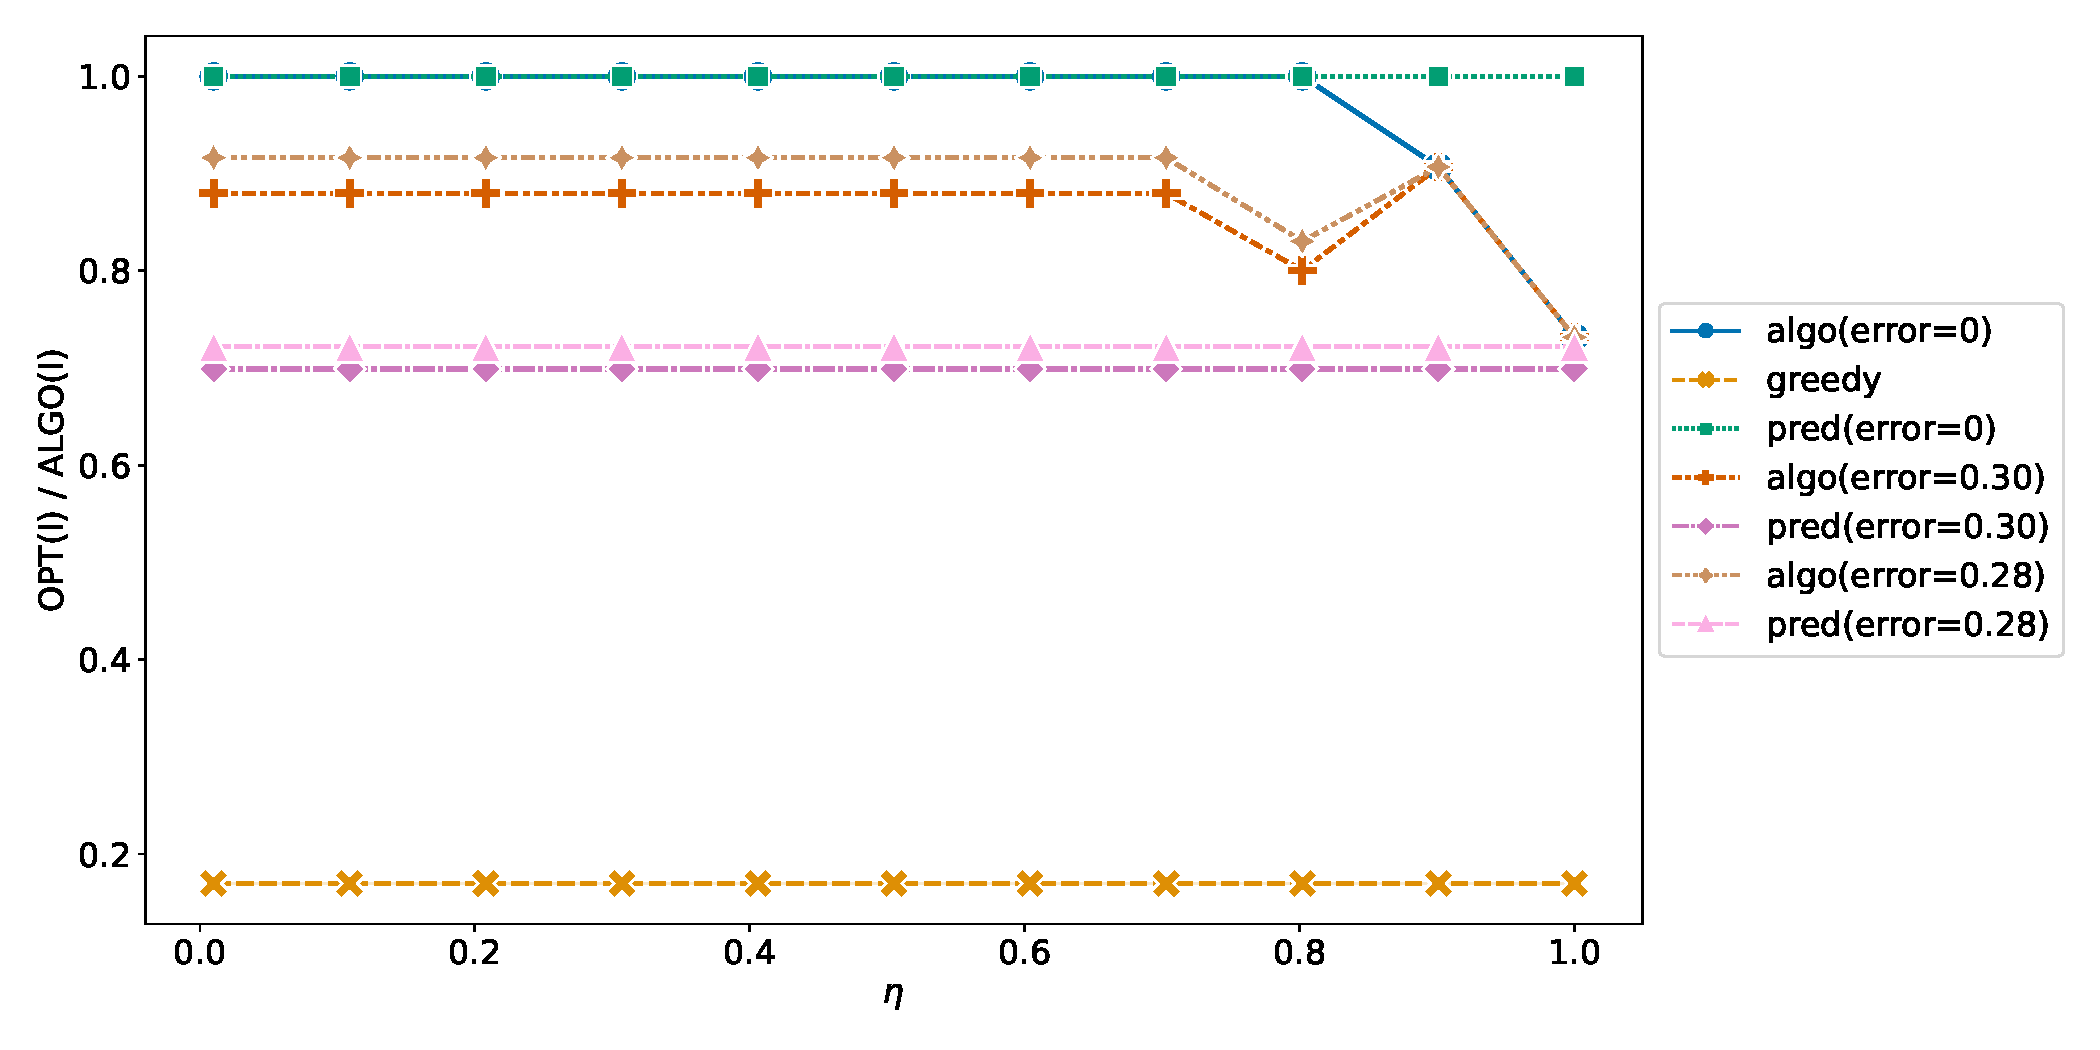
\includegraphics[width=\linewidth]{Img/figure2.pdf}
    \caption{Experiment result. The x-axis show the confidence in the prediction, where 0 means higher confidence. The y-axis show the competitive ratio compared to the optimal offline integral solution. The different colors (also markers) show the result of the algorithm with different prediction error rates and the solutions of the greedy algorithm and the prediction alone. The input graph has $20$ vertices, $69$ arcs, and $10$ requests.}
    \label{fig:experiment-2}
\end{figure}

\begin{figure}[!ht]
    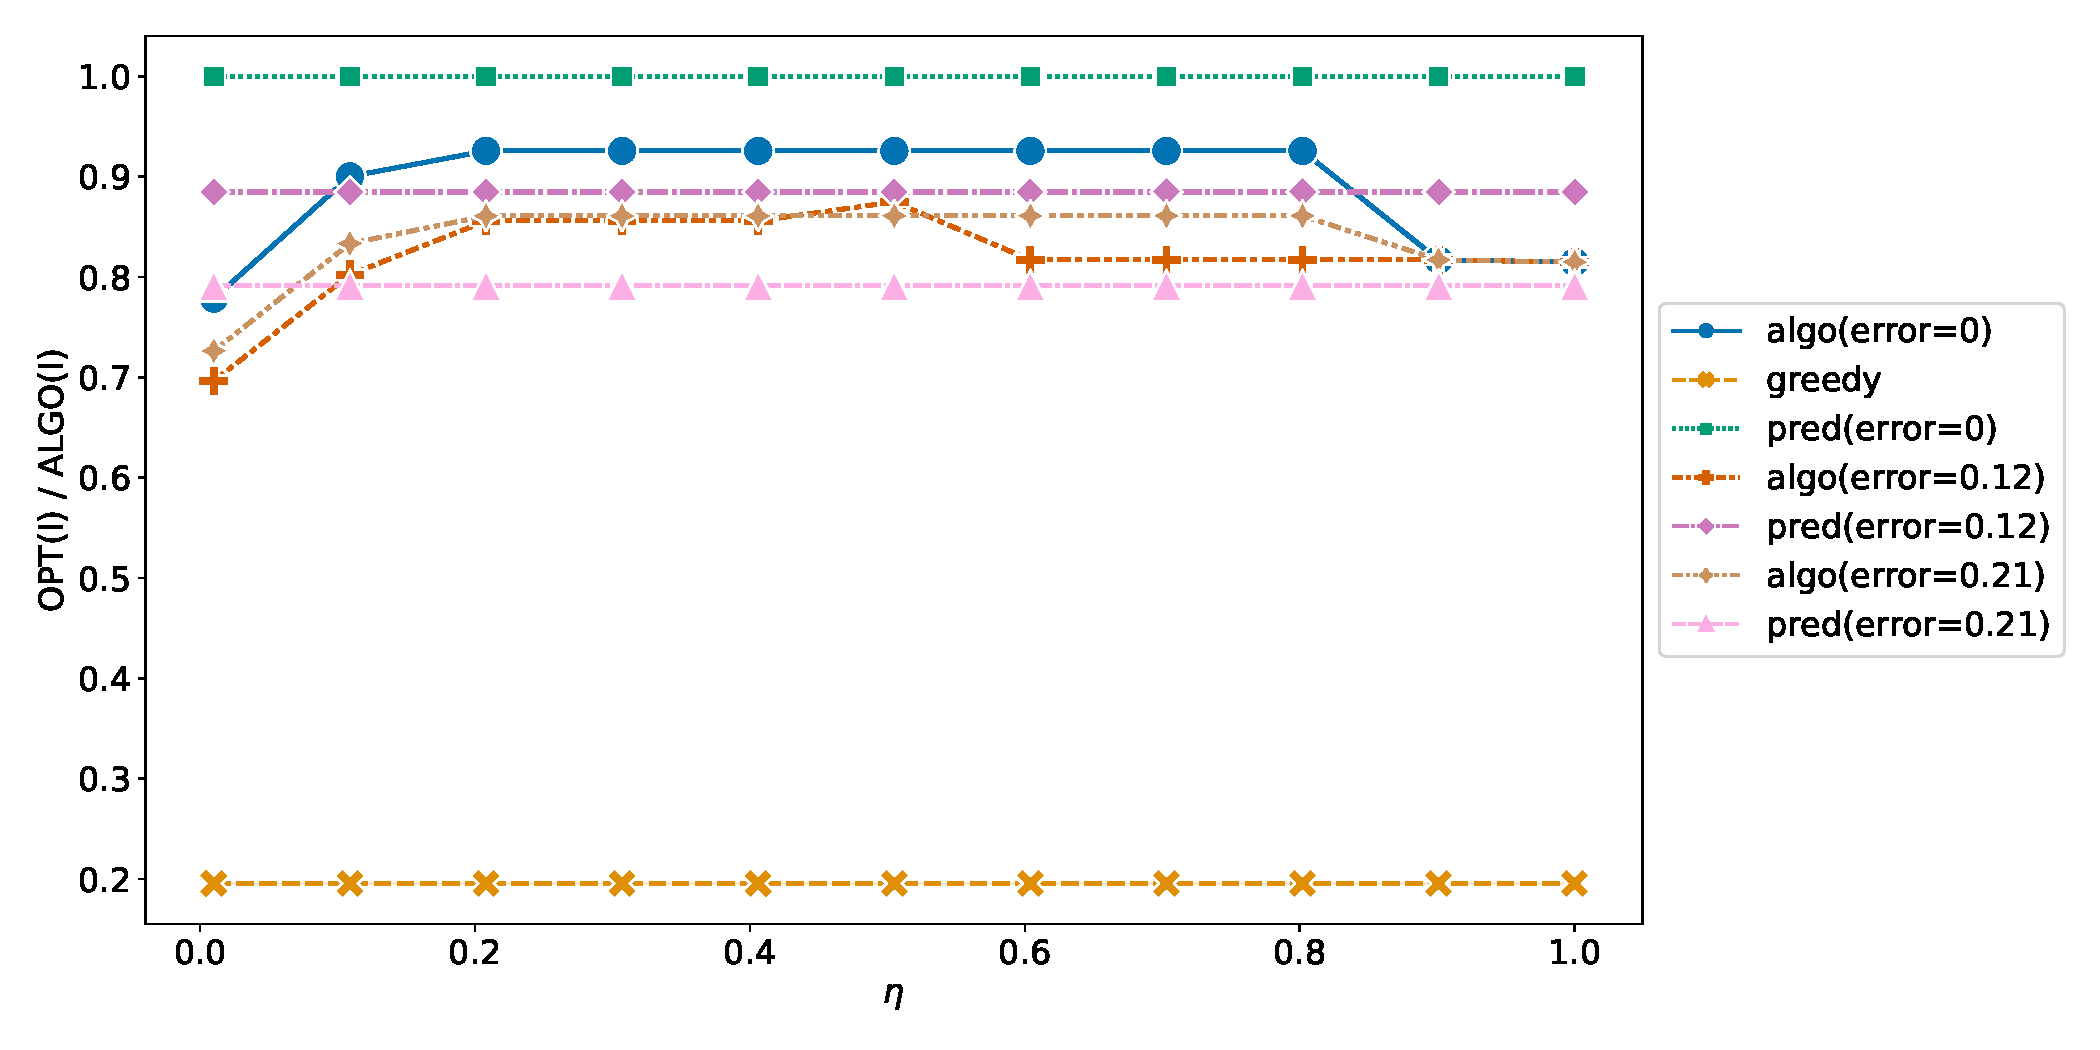
\includegraphics[width=\linewidth]{Img/figure3.pdf}
    \caption{Experiment result. The x-axis show the confidence in the prediction, where 0 means higher confidence. The y-axis show the competitive ratio compared to the optimal offline integral solution. The different colors (also markers) show the result of the algorithm with different prediction error rates and the solutions of the greedy algorithm and the prediction alone. The input graph has $30$ vertices, $73$ arcs, and $20$ requests.}
    \label{fig:experiment-3}
\end{figure}
